% LaTeX template for reports
% Author: Adam Jaamour
% Last updated: 13/04/2020

% ------------------- IMPORTS -------------------
\documentclass[letterpaper,12pt]{article}
\usepackage{tabularx} % extra features for tabular environment
\usepackage{amsmath}  % improve maths presentation
\usepackage{amssymb} % maths symbols
\usepackage{graphicx} % takes care of graphic including machinery
\usepackage[margin=0.95in,letterpaper]{geometry} % decreases margins
\usepackage{cite} % takes care of citations
\usepackage[titletoc,title]{appendix} % takes care of appendices
\usepackage{listings} % code representation
\usepackage{pdflscape}
\usepackage{csquotes} % for quoting existing work
\usepackage{color} % defines colours for code listings
\usepackage{comment} % allows for block of comments
\usepackage{gensymb} % degree symbol
\usepackage[table,xcdraw]{xcolor} % table colouring
\usepackage[cc]{titlepic}  % allows a pic to be included in the title page
\usepackage[final]{hyperref} % adds hyper links inside the generated pdf file
\usepackage{pdfpages} % include pdfs
\usepackage{subcaption} % subfigures to have multiple images on the same line

% ------------------- CODING STYLE -------------------
\definecolor{codegreen}{rgb}{0,0.6,0}
\definecolor{codegray}{rgb}{0.5,0.5,0.5}
\definecolor{backcolour}{rgb}{0.95,0.95,0.92}
\lstdefinestyle{mystyle}{
    backgroundcolor=\color{backcolour},   
    commentstyle=\color{codegreen},
    keywordstyle=\color{blue},
    numberstyle=\tiny\color{codegray},
    basicstyle=\footnotesize,
    breakatwhitespace=false,         
    breaklines=true,                 
    captionpos=b,                    
    keepspaces=true,                 
    numbersep=5pt,                  
    showspaces=false,                
    showstringspaces=false,
    showtabs=false,                  
    tabsize=4
}
\lstset{style=mystyle}

% ------------------- HEADINGS -------------------

\begin{document}

\title{
    CS5014 Machine Learning\\Practical 2 Report\\
    \begin{large}
    University of St Andrews - School of Computer Science
    \end{large}
}
\titlepic{
\includegraphics[width=0.3\linewidth]{figures/st-andrews-logo.jpeg}}
\author{Student ID: 150014151}
\date{5th May, 2020}
\maketitle
\newpage

\tableofcontents
\newpage

% ------------------- INTRODUCTION --------------------

\section{Introduction}
\label{sec:introduction}

This practical covers the exploration of various machine learning techniques used when dealing with real-life data. The data documents different types of seal pup found in cropped aerial imagery obtained during seasonal surveys of islands. Various data visualisation techniques, data processing steps and classification models are experimented with before designing a final pipeline to make predictions on the types of seals observed in the images. The predictions are made by training multiple classification models, which are all evaluated to determine their performance.\\

The report is separated in four sections, starting with a general introductory section before exploring the diverse array of methodologies and design decisions made during the development of the code in Python, followed by an evaluation of the final classifier and a critical reflection on the findings.

\subsection{Usage instructions}

Before running the code, create a new virtual environment and install the Python libraries used in the code by running the following command:

\begin{lstlisting}
pip install -r requirements.txt
\end{lstlisting}

To run the program, move to the “src” directory and run the following command:

\begin{lstlisting}
python main.py -s <section> -d <dataset> [-m <model>] [-g] [-v]
\end{lstlisting}

where:
\begin{itemize}
    \item``\textit{-s section}'': is a setting that executes different parts of the program. It must be one of the following: `\textit{data\_vis}', `\textit{train}' or `\textit{test}'.
    \item``\textit{-d dataset}'': selects the dataset to use. It must be set to either `\textit{binary}' or `\textit{multi}'.
    \item``\textit{-m model}'': is an optional setting that selects the classification model to use for training. It must be one of the following: `\textit{sgd}', `\textit{logistic}', `\textit{svc\_lin}', `\textit{svc\_poly}'.
    \item``\textit{-g}'': is an optional flag the grid search algorithm to determine the optimal hyperparameters for the selected regression model. The flag only takes effect when using XXX classifiers.
    \item``\textit{-v}'': is an optional flag that enters verbose (debugging) mode, printing additional statements on the command line.
\end{itemize}

\subsection{Tools used}

\begin{itemize}
    \item Programming language: Python 3.7.
    \item Python libraries used: SciKit-Learn\footnote{SciKit-Learn: \url{https://scikit-learn.org}}, Pandas\footnote{Pandas: \url{https://pandas.pydata.org/}}, Matplotlib\footnote{Matplotlib: \url{https://matplotlib.org/}}, NumPy\footnote{NumPy: \url{https://numpy.org/}} and Seaborn\footnote{Seaborn: \url{https://seaborn.pydata.org/}}.
    \item Editor: PyCharm\footnote{PyCharm: \url{https://www.jetbrains.com/pycharm/}}.
    \item Version controlling: Git and GitHub (private repository).
    \item Initial code prototyping: Jupyter Lab.
\end{itemize}

% ------------------- SYSTEM ARCHITECTURE --------------------

\section{System Architecture}
\label{sec:system-architecture}

\subsection{Project structure}

The project is organised into the following python modules:
\begin{itemize}
    \item `\textit{main.py}': 
    \item `\textit{data\_visualisation.py}': 
    \item `\textit{data\_manipulations.py}': 
    \item `\textit{classifiers.py}':
    \item `\textit{helpers.py}': 
    \item `\textit{config.py}': 
\end{itemize}

\subsection{Execution flow}

A command-line interface, implemented through Python’s native library \textit{argparse}\footnote{argparse: \url{https://docs.python.org/3.7/library/argparse.html}}, controls which dataset to use and which part of the program to run:
\begin{itemize}
    \item Visualising the data sets.
    \item Training different classification models.
    \item Running a grid search on selected models.
    \item Making predictions on the final model.
\end{itemize}

% ------------------- PART 3: XXXX --------------------

\section{Methodology \& data-driven design decisions}
\label{sec:methodology-design}

\subsection{Datasets}

\subsubsection{Data description}

The data comes in two flavours: \textit{binary} and \textit{multi}, where:
\begin{itemize}
    \item ``\textit{binary}'' data contains two labels, one for images of backgrounds and the other seals.
    \item ``\textit{multi}'' data contains five labels, one for images of backgrounds and the four others for types of seals (whitecoat, moulted pup, dead pup and juvenile).
\end{itemize}

\subsubsection{Data loading}

Each dataset contains three distinct CSV files:
\begin{itemize}
    \item ``\textit{X\_train.csv}'', containing the features of the images used for training which will be analysed in further sections.
    \item ``\textit{Y\_train.csv}'', containing the class label for each image.
    \item ``\textit{X\_test.csv}'', containing the features of the images used for testing. These will be used for making the final predictions with the optimal trained classifier.
\end{itemize}

The provided CSV files are directly loaded into distinct Pandas DataFrames\footnote{Pandas DataFrames: \url{https://pandas.pydata.org/pandas-docs/stable/reference/api/pandas.DataFrame.html}} by using the \textit{read\_csv} function. However, this method takes a long time due to the large file size (e.g. X\_train.csv is 1.5GB large). To speed up the process, the DataFrames are serialised and saved using Pickle\footnote{Pickle: \url{https://docs.python.org/3.7/library/pickle.html}}, boosting future loading times from X to X second.

% -------------------

\subsection{Data visualisation \& Analysis}

This data visualisation step\footnote{Note: running the code to visualise all the figures and tables produced takes roughly 80 seconds.} is crucial to understand the data and its underlying patterns before fitting a classification model to the training dataset.

\subsubsection{Data overview}

Storing the features and labels in Pandas \textit{DataFrames} provides a valuable array of functions that can be used to gain high-level insights on the data. Using the \textit{pandas.DataFrame.info} and \textit{pandas.DataFrame.describe} functions reveals important information such as:
\begin{itemize}
    \item There are 62210 images in the training set.
    \item There are 964 features describing each image.
    \item There are no missing values in the entire dataset as each feature has 62210 non-null values (number of images in the training set).
    \item All training values are numerical (floats).
\end{itemize}

This overview confirms that no data encoding is required to use the features, and that the data is ``clean'', requiring no further manipulation.

\subsubsection{Classes distribution}

As this is a classification task, it is important to verify the distribution of classes in the training  set to determine whether the data is skewed or not. This is achieved by plotting labels found in ``\textit{Y\_train.csv}'' in a bar chart.

\begin{figure}[h]
\centering
\begin{subfigure}{.5\textwidth}
  \centering
  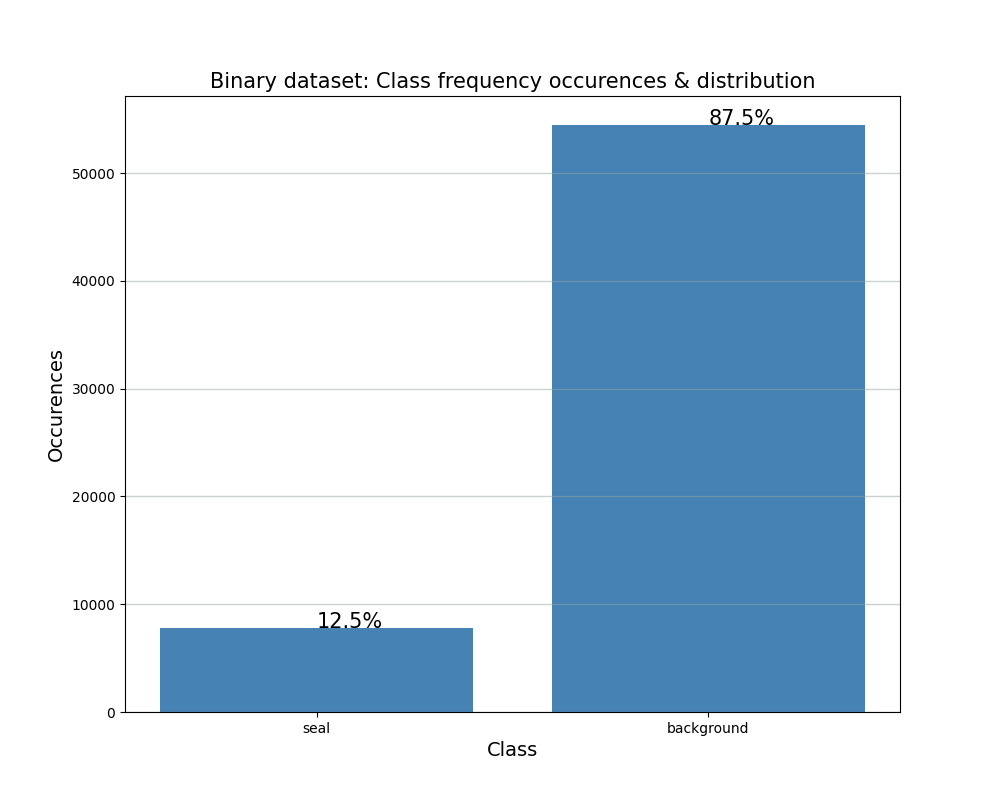
\includegraphics[width=\textwidth]{results/binary_class_distribution.png}
  \label{fig:binary_class_distribution}
\end{subfigure}%
\begin{subfigure}{.5\textwidth}
  \centering
  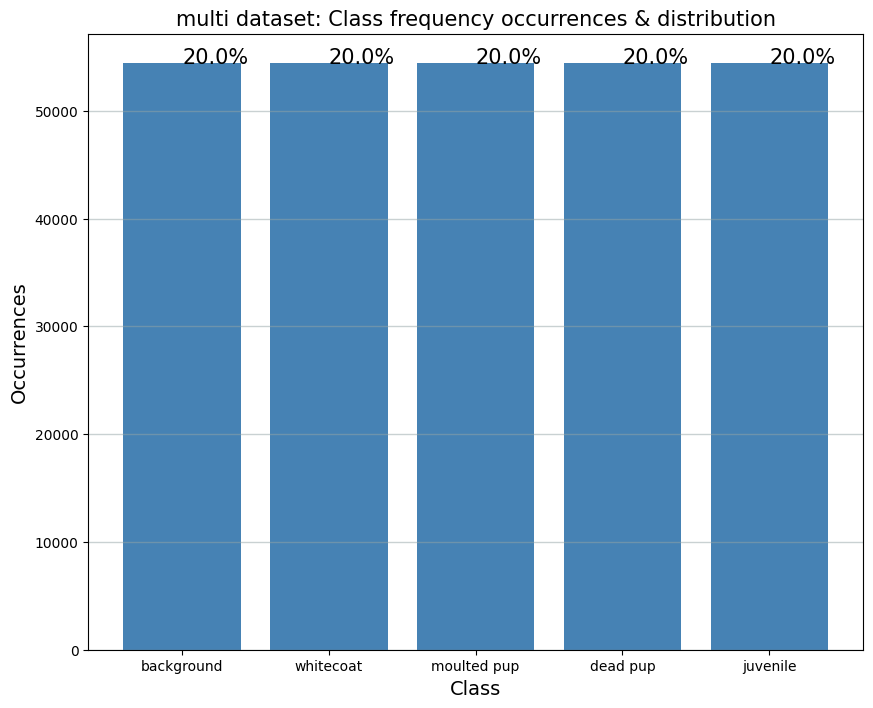
\includegraphics[width=\textwidth]{results/multi_class_distribution.png}
  \label{fig:multi_class_distribution}
\end{subfigure}
\caption{\label{fig:class_distribution}Class distribution of the binary (left) and multi (right) datasets.}
\end{figure}

These bar charts reveal that the dataset is heavily unbalanced, which must be taken into account when analysing the classifiers' scores. Indeed, using an  evaluation metric such as accuracy would be misleading as it would not be representative of how well the classifier fitted the data. For instance, if a dumb classifier that always classified an image as ``background'' was created, it would achieve 87.5\% accuracy. Therefore, other metrics such as confusion matrices, precision, recall and F1 scores could be used \cite{Geron2019}.

\subsubsection{Correlation}

There are three different types of features describing each image in the dataset:
\begin{itemize}
    \item Histogram of oriented Gradients (HoG), which correspond to a type of feature used in computer vision. The HoGs extracted from the datasets' images are histograms counting the occurrences of gradient orientations (9 orientations) in 2x2 blocks \cite{Dalal2005}. These correspond to the first 900 columns amongst the features dataset  in ``\textit{X\_train.csv}''.
    \item Samples from a normal distribution with parameters $\mu=0.5$ and $\sigma=2$. These correspond to columns 900 to 916 amongst the features dataset.
    \item 16-bin RGB colour histograms, corresponding to the last 48 columns in the features dataset.
\end{itemize}

Not all 964 features can be used due to the large complexity introduced by the number of dimensions the data has, also known as the curse of dimensionality \cite{Geron2019}. A preliminary check to determine which features can be considered ``important'' is conducted by calculating the standard correlation coefficient, a value ranging between -1 and 1, between the label (``\textit{Y\_train.csv}'') and all the features ``\textit{X\_train.csv}''. A value close to 1 indicates a strong positive linear correlation, while a correlation close to -1 indicates a strong negative linear correlation. However, a correlation close to 0 indicates a lack of relationship in the data. According to existing literature, features are considered to have a high correlation when they have values in the region of $[|0.5,0.7|]$ \cite{Geron2019} \cite{Badr2019}.\\

To determine which features show the highest correlation with the class labels, the \textit{pandas.DataFrame.corr} function is used on a concatenated DataFrame of the features and the labels. The ten features with the highest positive and negative correlation are shown in Figure \ref{fig:correlation-results}.

\begin{figure}[h]
\centering
\begin{subfigure}{.47\textwidth}
  \centering
  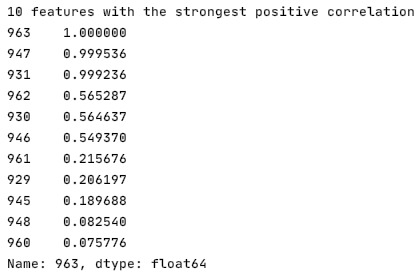
\includegraphics[width=\textwidth]{report/figures/corr_pos.png}
  \label{fig:corr_pos}
\end{subfigure}%
\begin{subfigure}{.5\textwidth}
  \centering
  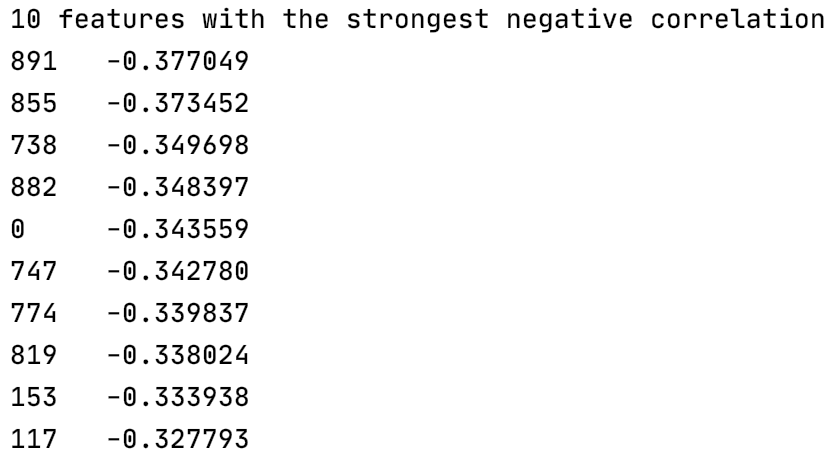
\includegraphics[width=\textwidth]{report/figures/corr_neg.png}
  \label{fig:corr_neg}
\end{subfigure}
\caption{\label{fig:correlation-results}Top 10 training dataset column indexes (features) with the highest standard correlation coefficient. Left shows positive correlations, right shows negative correlation.}
\end{figure}

High positive correlation is achieved for features ranging between columns 916-964, which corresponds to RGB colour histograms, while high negative correlation is achieved for features ranging between columns 0-900, which corresponds to HoGs. However, because no feature from the normal distribution have a high correlation  with the class labels, it can be dropped altogether.

\subsubsection{HoG features}

To directly visualise some information about the images, the HoG features can be reconstructed into images by being reshaped into 30x30 images, as seen in Figure \ref{fig:hog_multi}. Visualising the reconstructed HoG images confirms how it is impossible to discern the different classes with the human eye, and depicts how it will be impossible to infer anything from the reconstructed images of misclassified predictions.

\begin{figure}[h]
\centerline{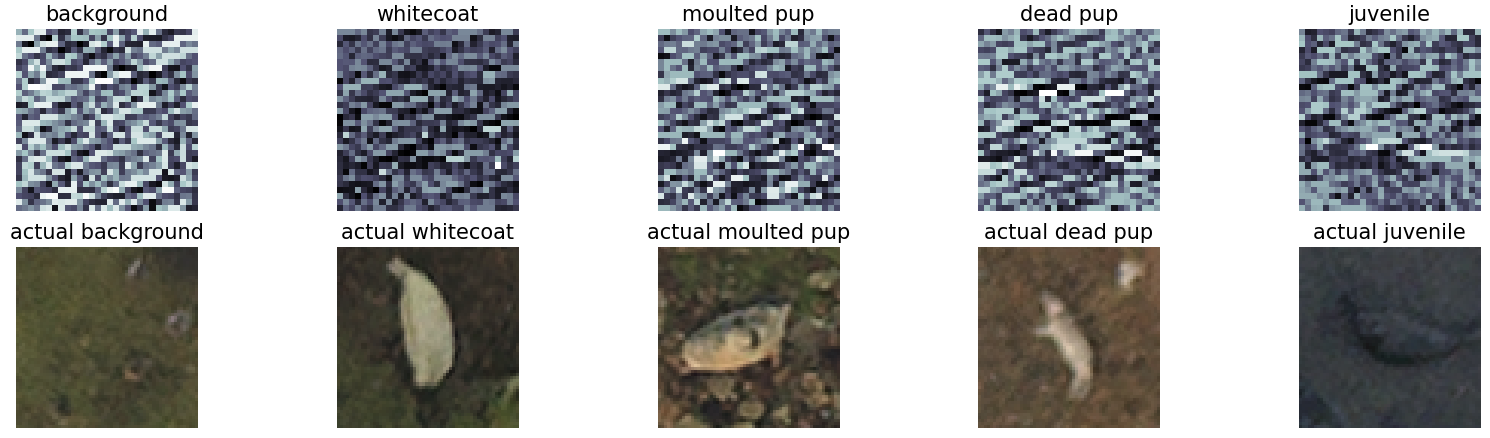
\includegraphics[width=\textwidth]{report/figures/hog_multi.png}}
\caption{\label{fig:hog_multi}Comparison of images reconstructed images from HoG features (top and middle rows) with actual images (bottom row).}
\end{figure}

\subsubsection{RGB colour histograms}

The features corresponding to the RGB colour histograms are visualised in Figure \ref{fig:rgb-hists}, revealing that there are more low-intensity pixels than high-intensity pixels. Because the range of values is considerable, the data will require some feature transformation such as standardising the dataset.

\begin{figure}[h]
\centering
\begin{subfigure}{.41\textwidth}
  \centering
  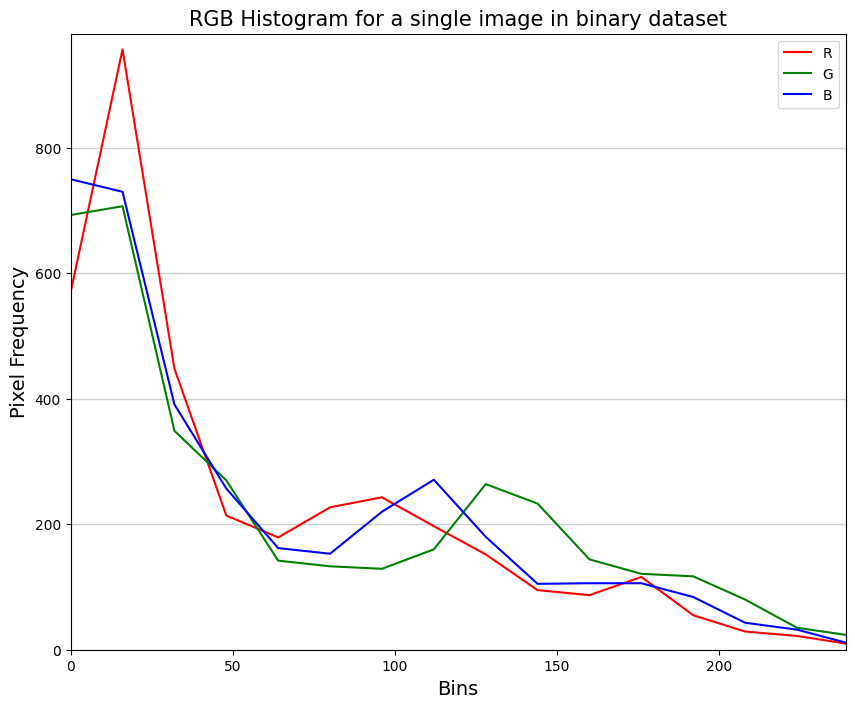
\includegraphics[width=\textwidth]{results/rgb_hist_single_image_binary.png}
  \label{fig:rgb_hist_single_image_binary}
\end{subfigure}%
\begin{subfigure}{.5\textwidth}
  \centering
  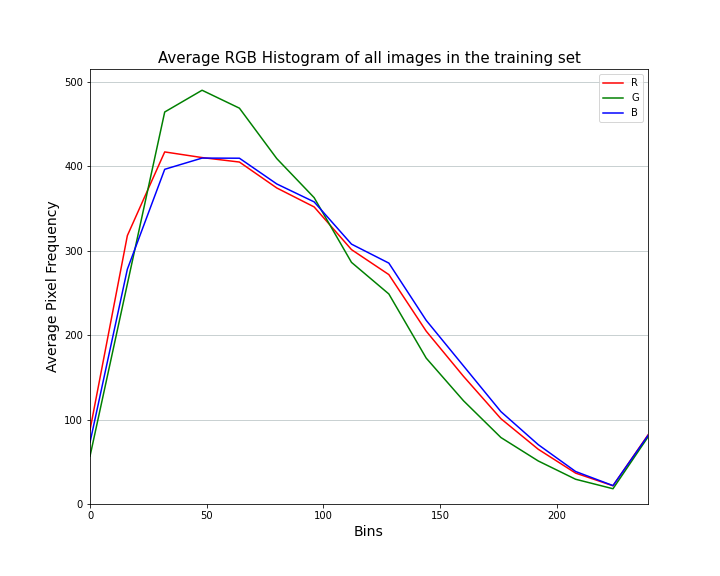
\includegraphics[width=\textwidth]{jupyter prototyping/rgb_avg_hist_all_training_set.png}
  \label{fig:rgb_avg_hist_all_training_set}
\end{subfigure}
\caption{\label{fig:rgb-hists}RGB histogram for a single random image (left) and average of all images in the training set (right).}
\end{figure}

% -------------------

\subsection{Input preparation}

With the data visualisation and analysis steps completed, the training set can now be pre-processed to maximise the classification models’ fit on the data. Based on the conclusions made from the data analysis, three pre-processing steps are carried out.\\

Based on the correlation results, the normal distribution features can be dropped from the training dataset. This brings down the number of dimensions in the training data from 964 to 948.\\

Next, visualising the values of the dataset revealed how the data distribution is not bell-shaped and has very different scales between the HoG features and the RGB histograms. Therefore, the features are standardised using the \textit{sklearn.preprocessing.StandardScaler} class, resulting in a distribution with unit variance a shape closer to a bell (the two properties of standardised distributions are a mean of all values equal to 0 and a standard deviation equal to 1) \cite{Geron2019}\cite{Glen2014}.\\

However, the curse of dimensionality remains as there are still 948 columns in the dataset. The most popular solution to counter this problem is to use Principal Component Analysis (PCA) to reduce the number of dimensions via projection. This is achieved by using the \textit{sklearn.decomposition.PCA} class. In order to choose the right number of dimensions to keep to preserve 99\% of the training set's explained variance, the explained variance is plotted against the number of dimensions in Figure \ref{fig:explained_variance}. The plot shows that to maintain 99\% variance, 487 can be kept, while diminishing the number of dimensions would reduce the variance under 99\%. The training set is therefore reduced to 487 dimensions, which is almost half the size of the original dataset \cite{Geron2019}.

\begin{figure}[h]
\centerline{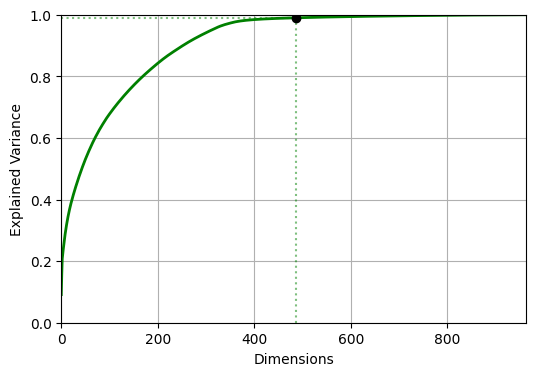
\includegraphics[width=0.6\textwidth]{report/figures/explained_variance.png}}
\caption{\label{fig:explained_variance}Explained variance plotted against number of dimensions. At least 487 dimensions are  required to maintain 99\% variance.}
\end{figure}

% -------------------

\subsection{Fitting}

\subsubsection{Strategy}

At this point, the training data is ready to be fed into the classifiers. The classification models will fit the features found in ``\textit{X\_train.csv}'' before making their own predictions, which will be compared with the real labels found in ``\textit{Y\_train.csv}'' for evaluation.\\

According to A. Géron, an efficient approach to model selection is to try out multiple classifiers, with hyperparameters close to the default values recommended by Scikit-Learn. The goal of this method is to gain a high-level intuition of which classification models to further explore and tweak \cite{Geron2019}. todo: mention which were chosen.

\subsubsection{Performance metrics}

todo

\subsubsection{K-fold cross validation}

todo

\subsection{Classification models}

SVC and logistic regression  don't natively work with multilabel classification, whereas SGD does.

\subsection{Model fine-tuning}

todo

\subsubsection{Training  execution flow}

todo

% ------------------- CONCLUSION --------------------

\section{Evaluation \& Critical discussion}
\label{sec:evaluation}

\subsection{Selecting the best classifier}

todo

\subsection{Final test}

todo

\subsection{Critical discussion}


% -------------------- APPENDIX --------------------

\begin{appendices}

\clearpage

\bibliographystyle{unsrt}
\bibliography{bibliography}

% --------------------

\clearpage
\section{Project Structure}
\label{sec:appendix-project-structure}

A screenshot of the project's file structure in the PyCharm IDE to illustrate the Python modules and data organisation.

add screenshot

% ------------------------

\end{appendices}
\end{document}